\documentclass[11pt,a4paper]{article}

% --- Geometry & Typography ---------------------------------------------------
\usepackage[a4paper,top=2.0cm,bottom=2.0cm,left=2.2cm,right=2.2cm,footskip=1.0cm,headsep=0.4cm]{geometry}
\usepackage[T1]{fontenc}
\usepackage[utf8]{inputenc}
\usepackage{lmodern}
\usepackage{microtype}
\usepackage[dvipsnames,table]{xcolor}
\usepackage{titlesec}
\usepackage{enumitem}
\usepackage{booktabs}
\usepackage{array}
\usepackage{tabularx}
\usepackage{caption}
\usepackage{amsmath,amssymb}
\usepackage{tikz}
\usetikzlibrary{positioning,arrows.meta,shapes.geometric,fit,backgrounds,calc,decorations.pathreplacing,decorations.pathmorphing}
\usepackage{pgfgantt}
\usepackage{float}
\usepackage{multicol}

% --- Color palette (extracted from pitching deck + WSO2 PDF) -----------------
\definecolor{neuroblue}{HTML}{1F2D7A}
\definecolor{accentpurple}{HTML}{5E2D91}
\definecolor{swrorange}{HTML}{D55E00}
\definecolor{nodepeach}{HTML}{FAD7C7}
\definecolor{nodeblue}{HTML}{CFE2F3}
\definecolor{nodegreen}{HTML}{D9EAD3}
\definecolor{rulegrey}{HTML}{8A8A8A}
\definecolor{nodelilac}{HTML}{E0CFE8}

% --- Bibliography (natbib + custom apalike-comma style) --------------------
\usepackage[round,authoryear,sort&compress]{natbib}
\bibliographystyle{apalike}
\setcitestyle{aysep={,}}

% --- Section title styling ---------------------------------------------------
\titleformat{\section}
  {\color{neuroblue}\sffamily\large\bfseries}{\thesection.}{0.5em}{}[\vspace{-0.3em}\textcolor{accentpurple}{\rule{\linewidth}{0.4pt}}]
\titleformat{\subsection}
  {\color{neuroblue}\sffamily\normalsize\bfseries}{\thesubsection}{0.5em}{}
\titlespacing*{\section}{0pt}{0.45em}{0.15em}
\titlespacing*{\subsection}{0pt}{0.25em}{0.05em}

% --- Spacing tweaks ----------------------------------------------------------
\setlength{\parskip}{0.15em}
\setlength{\parindent}{0pt}
\renewcommand{\arraystretch}{1.0}
\captionsetup{font=small,labelfont={bf,color=neuroblue},skip=2pt}

% --- Hyperref (load last) ----------------------------------------------------
\usepackage[hidelinks]{hyperref}
\hypersetup{
  colorlinks=true,linkcolor=neuroblue,citecolor=neuroblue,urlcolor=neuroblue,
  pdftitle={HippoCortex Research Proposal},
  pdfauthor={Group 07, University of Kelaniya}
}

% --- Custom commands ---------------------------------------------------------
\newcommand{\objbold}[1]{\textbf{\color{neuroblue}#1}}

\begin{document}
\pagestyle{plain}

% =============================================================================
% TITLE BAND (compact, not full-page)
% =============================================================================
\begin{center}
{\sffamily\LARGE\bfseries HippoCortex}\\[0.2em]
{\itshape\small Biologically-Inspired Continual Learning via Sharp Wave Ripple Generative Replay in State Space Models}\\[0.7em]
{\footnotesize
\setlength{\tabcolsep}{4pt}\renewcommand{\arraystretch}{1.0}
\begin{tabular*}{0.82\linewidth}{@{\extracolsep{\fill}}ll@{}}
Hasinthaka Piyumal~~{\small(SE/2021/036)} & Praveen Dedigama~~{\small(SE/2021/031)} \\
Induwara Mihisara~~{\small(SE/2021/025)}  & Thagya Kavindi~~{\small(SE/2021/062)} \\
\end{tabular*}
}\\[0.5em]
{\footnotesize Group 07 \quad\textperiodcentered\quad Supervisor: Dr.~Nalin Warnajith}\\[0.4em]
{\color{rulegrey}\rule{\linewidth}{0.4pt}}
\end{center}

% =============================================================================
% 1. INTRODUCTION
% =============================================================================
\section{Introduction}

\subsection{Background}
We want machines that can keep learning new things over time, the way people do. The problem is that today's neural networks forget. When you train them on a new task, they overwrite what they learned for the old one and their performance on it collapses~\citep{delange2022continual}. The field calls this \emph{catastrophic forgetting}~\citep{kirkpatrick2017overcoming}. Several workarounds exist, but none of them really fits a robot that has to keep learning for months on a small on-board computer.

\subsection{Importance}
A robot that ships with a frozen model cannot pick up a new room, a new object, or a new owner once it leaves the factory. Sending its data to a cloud server for re-training drains battery, leaks private camera footage, and does not work offline. If the robot can learn locally and its memory does not balloon as it sees more, we open the door to genuine lifelong adaptation for the next generation of personal and service robots.

\subsection{Motivation}
The mammalian brain has already solved this problem. While the animal is awake, the \emph{hippocampus} (a fast memory area) quickly stores new experience. Later, during sleep, it sends short \emph{compressed summaries} of those experiences to the \emph{neocortex} (a slower, long-term store) for safekeeping~\citep{buzsaki2015hippocampal,mcclelland1995complementary}. No raw recording is ever passed around. HippoCortex turns that idea into a system. We use a fast modern sequence model called Mamba~\citep{gu2023mamba} as the brain-like backbone, and instead of saving past data we keep tiny per-task summaries and let a small helper network recreate the missing experience whenever we need it.

% =============================================================================
% 2. PROBLEM STATEMENT
% =============================================================================
\section{Problem Statement}

Existing approaches to continual learning fall into three groups, and each one is a poor fit for a deployed robot. The \textbf{rehearsal} group keeps a buffer of past data, or trains a generator that recreates that data, and replays it~\citep{rebuffi2017icarl,shin2017continual}; storage and privacy costs grow as the robot sees more. The \textbf{regularisation} group adds a penalty that tries to stop important weights from changing~\citep{kirkpatrick2017overcoming}; the penalty is fragile to tune---too strong and the model stops learning, too weak and it forgets anyway. The \textbf{projection} group, including the recent state-space methods Mamba-CL~\citep{cheng2024mambacl} and Inf-SSM~\citep{lee2025exemplarfree}, asks the model to make all of its new learning in a "safe" direction that does not disturb older skills; this is light on memory but accuracy drops once the task stream gets long.

\textbf{No published method delivers all three of the following at once:} (i)~the model never stores raw past inputs; (ii)~the cost per training step is small enough that the method runs on a robot's on-board chip; and (iii)~accuracy stays competitive even after dozens of tasks. HippoCortex targets exactly this gap, by combining a tiny per-task summary, a small helper that recreates past experience from that summary, and a built-in safeguard that protects old skills during every weight update.

\subsection{Research questions}
The work is organised around four research questions.
\textbf{RQ1:} can a tiny per-task summary (a few statistics, kilobytes per task) really replace a buffer of past inputs without hurting accuracy on long task streams?
\textbf{RQ2:} can a small helper network recreate past experience from that summary closely enough that a classifier trained on the recreated experience transfers cleanly to real past inputs?
\textbf{RQ3:} does combining the two ideas above---compressed replay and a built-in safeguard against overwriting---do better than either idea on its own across twenty or more sequential tasks?
\textbf{RQ4:} does the resulting model fit the speed and memory budget of the Go2 Edu's on-board chip while running at well under 50\,ms per frame under a real-world task schedule?

% =============================================================================
% 3. OBJECTIVES
% =============================================================================
\section{Objectives}

\begin{enumerate}[label=\textbf{O\arabic*.},leftmargin=2.2em,itemsep=0.05em,topsep=0.1em]
  \item \objbold{Tiny per-task summary.} A small chunk of memory per task that captures the gist of what the network learned, without keeping any raw input. Target: the size of the summary stays the same regardless of how many training samples the task has.
  \item \objbold{Memory replay helper.} A small helper network that, given a task name, recreates synthetic versions of the experience the model had during that task. Target: a classifier trained on the recreated experience reaches within two percentage points of one trained on the real past data.
  \item \objbold{Built-in safeguard.} A simple step in training that catches changes which would damage what older tasks rely on and removes them before they reach the weights. Target: less than three percentage-point drop in old-task accuracy after twenty sequential tasks on Split-CIFAR100.
  \item \objbold{Validation on standard benchmarks.} Evaluate on two well-known continual-learning benchmarks (Split-CIFAR100 and ImageNet-R). Target: 8--10\% higher average accuracy than the closest published baseline (Mamba-CL) and around 4\% higher than the next one (Inf-SSM).
  \item \objbold{Robot deployment.} Add a Transformer-style block~\citep{vaswani2017attention} to handle camera input and run the whole system on the Unitree Go2 Edu robot. Target: each frame processed in under 50\,ms on the robot's on-board chip.
  \item \objbold{Publication.} Two peer-reviewed papers: one on the Stage~1 algorithm, one on the Stage~2 robot deployment.
\end{enumerate}

% =============================================================================
% 4. PRELIMINARY LITERATURE REVIEW
% =============================================================================
\section{Preliminary Literature Review}

\subsection{Catastrophic forgetting}
\citet{kirkpatrick2017overcoming} introduced the most-cited modern fix, Elastic Weight Consolidation. The idea is to ask the network to keep its weights close to where they ended up after the previous task, with extra resistance to changing the weights that mattered most for that task. It works on short task streams but starts to misbehave as tasks pile up~\citep{delange2022continual}.

\subsection{Rehearsal and generative replay}
iCaRL~\citep{rebuffi2017icarl} simply keeps a small buffer of past examples and rehearses them along with the new task; storage grows with the number of classes seen. Deep Generative Replay~\citep{shin2017continual} replaces the buffer with a generator that recreates past inputs, but training a high-quality image generator on the fly on an edge device is not realistic. HippoCortex follows the same generative-replay idea but recreates the model's \emph{internal experience} instead of the raw image, which keeps the helper network small enough to run on the robot.

\subsection{Methods that protect old skills directly}
A second line of work asks the model to make every weight update in a direction that simply cannot disturb what older tasks relied on~\citep{saha2021gradient}. The recent state-space variants Mamba-CL~\citep{cheng2024mambacl} and Inf-SSM~\citep{lee2025exemplarfree} apply the same idea to fast modern sequence models. They keep no buffer at all, but their accuracy still slips on long task streams. HippoCortex adds the recreated-experience signal on top of this safeguard, so the two mechanisms cover each other's weaknesses.

\subsection{Modern sequence models}
Mamba~\citep{gu2023mamba} is a recent sequence model that matches Transformer-quality accuracy while running in linear time and using a small, constant amount of memory per step. That is exactly the profile we need on a robot: long memory of past observations without the heavy cost that attention-based models pay.

\subsection{Biological grounding}
\citet{buzsaki2015hippocampal} reviews twenty years of evidence that the hippocampus replays its memories during sleep, and \citet{mcclelland1995complementary} explains why a fast memory and a slow memory together avoid interference: they exchange short summaries, not the raw experience itself. HippoCortex copies the same division of labour (Figure~\ref{fig:biomap}).

\subsection{Research gap}
Across the strands above, no published method offers all of: no raw data stored, fast on-device training, and stable accuracy after many sequential tasks, all validated on a real robot. Figure~\ref{fig:methodtable} lays out the gap HippoCortex fills.

% --- FIGURE 1: Bio mapping ---------------------------------------------------
\begin{figure}[ht]
\centering
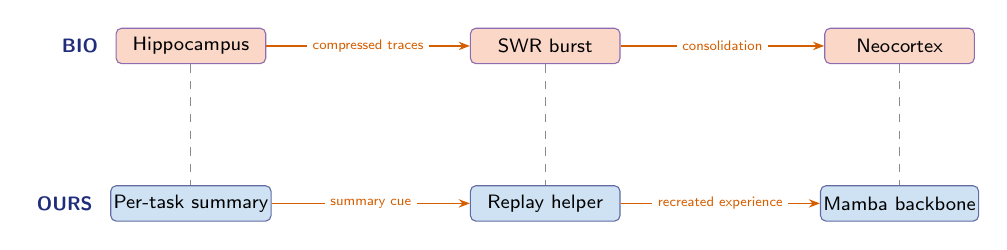
\begin{tikzpicture}[
  font=\sffamily\scriptsize,
  bionode/.style={rectangle,rounded corners=2pt,draw=accentpurple!70,fill=nodepeach,minimum width=1.9cm,minimum height=0.45cm,inner sep=1pt},
  cmpnode/.style={rectangle,rounded corners=2pt,draw=neuroblue!70,fill=nodeblue,minimum width=1.9cm,minimum height=0.45cm,inner sep=1pt},
  arr/.style={-{Stealth[length=4pt]},semithick,swrorange},
  dashlink/.style={dashed,thin,rulegrey},
  lanelabel/.style={font=\sffamily\scriptsize\bfseries,text=neuroblue},
  arrlabel/.style={font=\sffamily\tiny,text=swrorange,fill=white,inner xsep=2pt,inner ysep=0.5pt},
]
% Bio lane (top)
\node[bionode] (hipp)   at (0.5,1.5)  {Hippocampus};
\node[bionode] (swr)    at (5.0,1.5)  {SWR burst};
\node[bionode] (cortex) at (9.5,1.5)  {Neocortex};
\node[lanelabel,anchor=east] at ($(hipp.west)+(-0.1,0)$) {BIO};
\draw[arr] (hipp) -- node[arrlabel]{compressed traces} (swr);
\draw[arr] (swr)  -- node[arrlabel]{consolidation} (cortex);

% Computational lane (bottom)
\node[cmpnode] (sb)    at (0.5,-0.5) {Per-task summary};
\node[cmpnode] (gen)   at (5.0,-0.5) {Replay helper};
\node[cmpnode] (mamba) at (9.5,-0.5) {Mamba backbone};
\node[lanelabel,anchor=east] at ($(sb.west)+(-0.1,0)$) {OURS};
\draw[arr] (sb)  -- node[arrlabel]{summary cue} (gen);
\draw[arr] (gen) -- node[arrlabel]{recreated experience} (mamba);

% Vertical analogy links
\draw[dashlink] (hipp)   -- (sb);
\draw[dashlink] (swr)    -- (gen);
\draw[dashlink] (cortex) -- (mamba);
\end{tikzpicture}
\caption{Mapping of biological consolidation onto HippoCortex components.}
\label{fig:biomap}
\end{figure}

% --- FIGURE 2: Method comparison table-as-figure -----------------------------
\begin{figure}[ht]
\centering
\footnotesize
\setlength{\tabcolsep}{4pt}
\begin{tabular*}{\linewidth}{@{\extracolsep{\fill}}lcccc@{}}
\toprule
\textbf{Method} & \textbf{Replay style} & \textbf{Raw data?} & \textbf{Memory growth} & \textbf{On robot?} \\
\midrule
EWC~\citep{kirkpatrick2017overcoming}              & none                & no             & small but task-aware  & no \\
iCaRL~\citep{rebuffi2017icarl}                     & real past examples  & \textbf{yes}   & grows with classes    & no \\
DGR~\citep{shin2017continual}                      & recreates raw pixels & no            & generator-sized       & no \\
GPM~\citep{saha2021gradient}                       & none, safeguard only & no            & grows with tasks      & no \\
Mamba-CL~\citep{cheng2024mambacl}                  & none, safeguard only & no            & grows with tasks      & no \\
Inf-SSM~\citep{lee2025exemplarfree}                & none, safeguard only & no            & grows with tasks      & no \\
\rowcolor{nodegreen}\textbf{\color{neuroblue}HippoCortex (ours)} & \textbf{\color{neuroblue}internal experience + safeguard} & \textbf{\color{neuroblue}no} & \textbf{\color{neuroblue}few KB per task} & \textbf{\color{neuroblue}yes (Go2)} \\
\bottomrule
\end{tabular*}
\caption{Comparison of continual-learning methods. HippoCortex is the only entry that combines latent generative replay with null-space protection on a linear-time SSM backbone, with planned validation on a physical robot.}
\label{fig:methodtable}
\end{figure}

% =============================================================================
% 5. METHODOLOGY
% =============================================================================
\section{Methodology}

The project runs in two stages. \textbf{Stage 1} (Months 1--3) builds the core algorithm and validates it on standard image benchmarks. \textbf{Stage 2} (Months 4--10) extends the model to a hybrid architecture and deploys it on the Unitree Go2 Edu quadruped. Hardware access for Stage 2 is already in hand: the team's separate hardware proposal to the WSO2 Call for Proposals on Unitree Go2 Edu Robot-based Projects has been \emph{approved}, which gives us access to the robot at the WSO2 Colombo office along with a project grant.

\subsection{Stage 1: Core system (Months 1--3)}
HippoCortex chains four pieces, shown in Figure~\ref{fig:pipeline}:
\begin{itemize}[leftmargin=1.4em,itemsep=0.05em,topsep=0.1em]
  \item \textbf{Mamba backbone.} A fast modern sequence network~\citep{gu2023mamba} that does the actual learning.
  \item \textbf{Per-task summary.} A tiny record we keep about each task we have seen, capturing only what the model's internal features looked like for that task. We never keep raw images.
  \item \textbf{Replay helper.} A small generator network~\citep{sohn2015learning} that, given a task name, recreates how the backbone's internals would have looked during that task.
  \item \textbf{Built-in safeguard.} A simple step that we apply on every weight update. It catches the part of the update that would hurt older skills and removes it before the update is applied~\citep{saha2021gradient,cheng2024mambacl}.
\end{itemize}

\textbf{Training loop (per new task).} For each new task we run three short passes. (i)~A \emph{warm-up} on the new task alone, so the backbone gets a sensible starting point. (ii)~A \emph{joint pass} mixes the new task with recreated past experience from the replay helper, and routes every weight update through the safeguard. (iii)~A \emph{consolidation} pass updates the per-task summary with the new task and tells the safeguard which directions to protect from now on.

\textbf{Benchmarks, baselines, metrics.}

\begin{center}\small
\begin{tabular}{@{}l p{0.74\linewidth}@{}}
\toprule
\textbf{Datasets}   & Split-CIFAR100 (twenty 5-class tasks) and ImageNet-R (a harder distribution shift). \\
\textbf{Baselines}  & Naive fine-tuning, EWC~\citep{kirkpatrick2017overcoming}, DGR~\citep{shin2017continual}, Mamba-CL~\citep{cheng2024mambacl}, Inf-SSM~\citep{lee2025exemplarfree}. \\
\textbf{Metrics}    & Average accuracy across tasks, forgetting rate, and memory used (in MB) as the number of tasks grows. \\
\bottomrule
\end{tabular}
\end{center}

% --- FIGURE 3: Stage 1 pipeline ---------------------------------------------
\begin{figure}[ht]
\centering
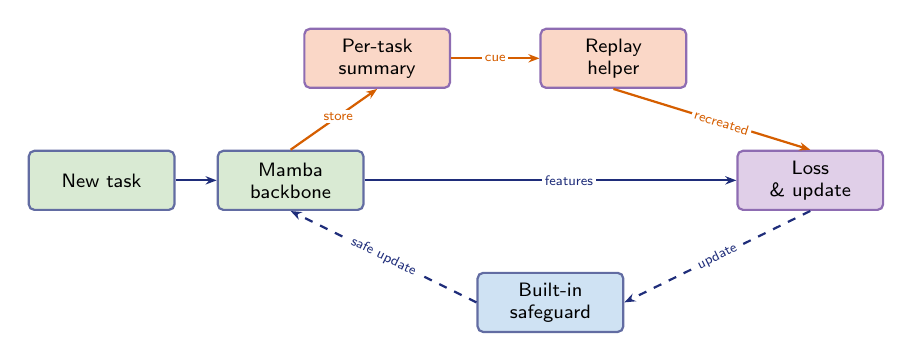
\begin{tikzpicture}[
  font=\sffamily\scriptsize,
  block/.style={rectangle,rounded corners=2pt,draw,thick,minimum height=0.75cm,minimum width=1.85cm,align=center,inner sep=2pt},
  inn/.style={block,fill=nodegreen,draw=neuroblue!70},
  buf/.style={block,fill=nodepeach,draw=accentpurple!70},
  proj/.style={block,fill=nodeblue,draw=neuroblue!70},
  term/.style={block,fill=nodelilac,draw=accentpurple!70},
  arr/.style={-{Stealth[length=4pt]},thick,neuroblue},
  swr/.style={-{Stealth[length=4pt]},thick,swrorange},
  fwdlbl/.style={font=\sffamily\tiny,text=neuroblue,fill=white,inner sep=1pt},
  swrlbl/.style={font=\sffamily\tiny,text=swrorange,fill=white,inner sep=1pt},
  graddlbl/.style={font=\sffamily\tiny,text=neuroblue,fill=white,inner sep=1pt},
]
% Top row: replay path
\node[buf] (sb)    at (3.5, 1.55) {Per-task\\summary};
\node[buf] (gen)   at (6.5, 1.55) {Replay\\helper};
% Middle row: forward path
\node[inn] (input) at (0,    0)   {New task};
\node[inn] (mamba) at (2.4,  0)   {Mamba\\backbone};
\node[term] (loss) at (9.0,  0)   {Loss\\\& update};
% Bottom row: projection
\node[proj] (proj) at (5.7, -1.55){Built-in\\safeguard};

% Forward pass (blue, solid)
\draw[arr] (input) -- (mamba);
\draw[arr] (mamba.east) -- node[fwdlbl,pos=0.55]{features} (loss.west);

% Replay path (orange, solid) -- straight diagonals, labels in open space
\draw[swr] (mamba.north) -- node[swrlbl,pos=0.55]{store} (sb.south);
\draw[swr] (sb.east) -- node[swrlbl]{cue} (gen.west);
\draw[swr] (gen.south) -- node[swrlbl,sloped,pos=0.55]{recreated} (loss.north);

% Gradient projection (dashed, blue) -- diagonals
\draw[arr,dashed] (loss.south) -- node[graddlbl,sloped,pos=0.5]{update} (proj.east);
\draw[arr,dashed] (proj.west) -- node[graddlbl,sloped,pos=0.5]{safe update} (mamba.south);
\end{tikzpicture}
\caption{The Stage 1 HippoCortex system. Recreated past experience from the replay helper is mixed with the current task; every weight update passes through the safeguard before reaching the backbone, so older skills stay intact.}
\label{fig:pipeline}
\end{figure}

\subsection{Stage 2: Robot deployment (Months 4--6)}
The Mamba backbone alone does not make full use of spatial structure in camera frames, so for the robot we add a Transformer-style block~\citep{vaswani2017attention} between two Mamba layers. The Mamba layers handle the time dimension (the stream of frames), and the attention block helps with the visual content of each frame. The same HippoCortex safeguard and replay helper wrap the whole thing, so we do not need to change anything else. The model runs on the Go2 Edu's on-board chip (Jetson Orin NX 16\,GB, 100 TOPS). On the robot we test it on four tasks back-to-back: recognising terrain, interacting with an object, staying aware of nearby people, and mapping a new room. The implementation uses standard tools: Python~3.11, PyTorch~2.x, ROS2, and Mujoco / Isaac~Sim for pre-deployment testing in simulation.

% =============================================================================
% 6. EXPECTED PROJECT DELIVERABLES
% =============================================================================
\section{Expected Project Deliverables}

\begin{itemize}[leftmargin=1.4em,itemsep=0.0em,topsep=0.05em]
  \item \objbold{Open-source reference implementation} (PyTorch, GitHub) of the full HippoCortex stack with reproducible training scripts and pre-trained checkpoints.
  \item \objbold{Stage 1 benchmark report} on Split-CIFAR100 and ImageNet-R: average accuracy, forgetting rate, memory footprint, and full per-component ablations against EWC, DGR, Mamba-CL and Inf-SSM.
  \item \objbold{Stage 1 paper} (peer-reviewed) describing the core algorithm and Stage 1 results.
  \item \objbold{Hybrid Mamba + Transformer extension} that wraps the SWR module around the hybrid stack for richer visual input.
  \item \objbold{Embodied demonstration} on the Go2 Edu running the four-task curriculum (terrain, object interaction, human proximity, environment mapping) on-device, with logged latency and per-task accuracy.
  \item \objbold{Stage 2 paper and thesis chapter} documenting the full embodied evaluation.
\end{itemize}

% =============================================================================
% 7. PROJECT SCHEDULE
% =============================================================================
\section{Project Schedule}

% --- FIGURE 5: Gantt (Apr 2026 -- Sep 2026, twelve half-month columns) -----
\begin{figure}[!ht]
\centering
\begin{ganttchart}[
  hgrid={*1{draw=gray!30,thin}},
  vgrid={*1{draw=gray!30,very thin}},
  x unit=0.78cm,
  y unit chart=0.42cm,
  y unit title=0.5cm,
  bar height=0.62,
  bar top shift=0.18,
  bar/.append style={draw=neuroblue!80,fill=neuroblue!35,rounded corners=1.5pt},
  bar label font=\sffamily\scriptsize,
  bar label node/.append style={align=right,text width=5.5cm},
  group/.append style={draw=accentpurple,fill=accentpurple!55,rounded corners=1.5pt},
  group label font=\sffamily\scriptsize\bfseries,
  group label node/.append style={text=accentpurple},
  group peaks width=0,
  group peaks height=0,
  group left shift=0,
  group right shift=0,
  group top shift=0.15,
  group height=0.7,
  milestone/.append style={fill=swrorange,draw=swrorange!70!black},
  milestone label font=\sffamily\tiny\bfseries,
  milestone label node/.append style={text=swrorange!70!black},
  milestone height=0.5,
  milestone top shift=0.25,
  title label font=\sffamily\scriptsize\bfseries,
  title/.append style={draw=accentpurple!70,fill=accentpurple!10},
  title height=1,
  ]{1}{12}
  \gantttitle{Apr 2026}{2} \gantttitle{May}{2} \gantttitle{Jun}{2} \gantttitle{Jul}{2} \gantttitle{Aug}{2} \gantttitle{Sep 2026}{2} \\
  \ganttgroup{Stage 1: Core algorithm}{1}{6} \\
  \ganttbar{T1 Literature review \& knowledge base}{1}{2} \\
  \ganttbar{T2 Proposal development \& submission}{1}{2} \\
  \ganttbar{T3 Stage 1 core: Mamba + projector}{2}{3} \\
  \ganttbar{T4 Stage 1 replay: stats buffer + SWR generator}{3}{4} \\
  \ganttbar{T5 Stage 1 benchmarking \& ablations}{4}{5} \\
  \ganttbar{T6 Stage 1 paper draft \& submission}{5}{6} \ganttmilestone[inline=false]{}{6} \\
  \ganttgroup{Stage 2: Embodied deployment}{6}{12} \\
  \ganttbar{T7 Hybrid Mamba + Transformer}{6}{7} \\
  \ganttbar{T8 Simulator integration \& curriculum}{7}{9} \\
  \ganttbar{T9 Robot deployment on Go2 Edu}{8}{11} \\
  \ganttbar{T10 Real-world experiments}{11}{11} \\
  \ganttbar{T11 Stage 2 paper \& thesis}{10}{12} \ganttmilestone[inline=false]{}{12}
\end{ganttchart}\\[0.2em]
\hspace*{6.0cm}\textcolor{swrorange!70!black}{\sffamily\tiny\bfseries$\blacklozenge$~Paper 1 (mid Jun)\quad$\blacklozenge$~Paper 2 + release (mid Sep)}
\caption{Six-month project schedule (April--September 2026). Each column is a half-month. Stage 1 delivers the core algorithm and first paper by late June; Stage 2 covers the hybrid extension, simulator validation, on-device robot deployment, real-world experiments, and the final paper / thesis.}
\label{fig:gantt}
\end{figure}

\subsection{Team responsibilities}
The Gantt above lists each task's lead. Per-member ownership is summarised below.

\begin{center}\small
\begin{tabularx}{\linewidth}{@{}l l X@{}}
\toprule
\textbf{Member} & \textbf{ID} & \textbf{Primary responsibility} \\
\midrule
Hasinthaka Piyumal & SE/2021/036 & Team lead, research direction, training pipeline, paper writing, WSO2 liaison. \\
Praveen Dedigama   & SE/2021/031 & Mamba backbone, null-space projector, hybrid stack design. \\
Induwara Mihisara  & SE/2021/025 & Biological grounding, data loaders, simulator integration. \\
Thagya Kavindi     & SE/2021/062 & Evaluation metrics, benchmark runs, ablation studies, results analysis. \\
\bottomrule
\end{tabularx}
\end{center}

% =============================================================================
% 7. REFERENCES
% =============================================================================
\section{References}
{\footnotesize
\setlength{\bibsep}{0.05em}
\renewcommand{\section}[2]{}% suppress duplicate heading produced by thebibliography
\begin{thebibliography}{12}
\bibitem[Buzs\'aki, 2015]{buzsaki2015hippocampal}
Buzs\'aki, G. (2015). Hippocampal sharp wave-ripple: A cognitive biomarker for episodic memory and planning. \emph{Hippocampus}, 25(10), 1073--1188.

\bibitem[Cheng et al., 2024]{cheng2024mambacl}
Cheng, D., Huang, Y., Zhang, J., Chen, K., Liu, M., \& Huang, Q. (2024). Mamba-CL: Optimizing selective state space model in null space for continual learning. \emph{arXiv preprint arXiv:2411.15469}.

\bibitem[De Lange et al., 2022]{delange2022continual}
De Lange, M., Aljundi, R., Masana, M., Parisot, S., Jia, X., Leonardis, A., Slabaugh, G., \& Tuytelaars, T. (2022). A continual learning survey: Defying forgetting in classification tasks. \emph{IEEE Transactions on Pattern Analysis and Machine Intelligence}, 44(7), 3366--3385.

\bibitem[Gu \& Dao, 2023]{gu2023mamba}
Gu, A., \& Dao, T. (2023). Mamba: Linear-time sequence modeling with selective state spaces. \emph{arXiv preprint arXiv:2312.00752}.

\bibitem[Kirkpatrick et al., 2017]{kirkpatrick2017overcoming}
Kirkpatrick, J., Pascanu, R., Rabinowitz, N., Veness, J., Desjardins, G., Rusu, A.~A., Milan, K., Quan, J., Ramalho, T., Grabska-Barwinska, A., Hassabis, D., Clopath, C., Kumaran, D., \& Hadsell, R. (2017). Overcoming catastrophic forgetting in neural networks. \emph{Proceedings of the National Academy of Sciences}, 114(13), 3521--3526.

\bibitem[Lee et al., 2025]{lee2025exemplarfree}
Lee, I.~N., Mahmoodi, L., Le, T., \& Harandi, M. (2025). Exemplar-free continual learning for state space models. \emph{arXiv preprint arXiv:2505.18604}.

\bibitem[McClelland et al., 1995]{mcclelland1995complementary}
McClelland, J.~L., McNaughton, B.~L., \& O'Reilly, R.~C. (1995). Why there are complementary learning systems in the hippocampus and neocortex: Insights from the successes and failures of connectionist models of learning and memory. \emph{Psychological Review}, 102(3), 419--457.

\bibitem[Rebuffi et al., 2017]{rebuffi2017icarl}
Rebuffi, S.-A., Kolesnikov, A., Sperl, G., \& Lampert, C.~H. (2017). iCaRL: Incremental classifier and representation learning. In \emph{Proceedings of the IEEE Conference on Computer Vision and Pattern Recognition (CVPR)} (pp.~2001--2010).

\bibitem[Saha et al., 2021]{saha2021gradient}
Saha, G., Garg, I., \& Roy, K. (2021). Gradient projection memory for continual learning. In \emph{International Conference on Learning Representations (ICLR)}.

\bibitem[Shin et al., 2017]{shin2017continual}
Shin, H., Lee, J.~K., Kim, J., \& Kim, J. (2017). Continual learning with deep generative replay. In \emph{Advances in Neural Information Processing Systems (NeurIPS)}.

\bibitem[Sohn et al., 2015]{sohn2015learning}
Sohn, K., Lee, H., \& Yan, X. (2015). Learning structured output representation using deep conditional generative models. In \emph{Advances in Neural Information Processing Systems (NeurIPS)}.

\bibitem[Vaswani et al., 2017]{vaswani2017attention}
Vaswani, A., Shazeer, N., Parmar, N., Uszkoreit, J., Jones, L., Gomez, A.~N., Kaiser, \L., \& Polosukhin, I. (2017). Attention is all you need. In \emph{Advances in Neural Information Processing Systems (NeurIPS)}.
\end{thebibliography}
}

\end{document}
